\begin{figure*}[t]
\centering
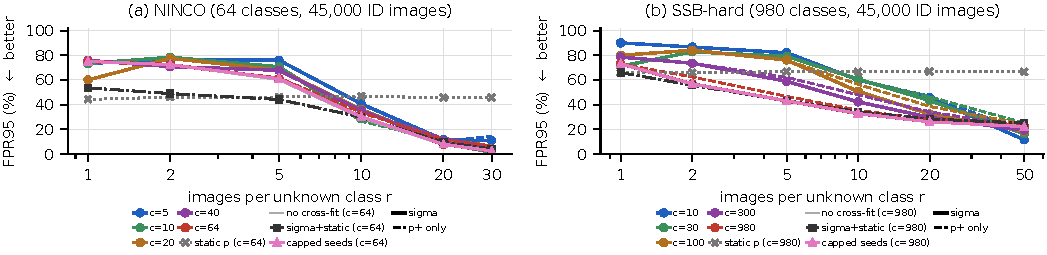
\includegraphics[width=\textwidth]{figs/fig18_rec.pdf}
\caption{再出現と混入率（\FPR{}，単体，DINOv2 L/14 + DINOv3 L/16）．IDの検証画像45,000枚に，NINCO（a）またはSSB-hard（b）から$c$個の未知クラス$\times$$r$枚を加えたテスト集合（クラスと画像の選び方を変えた3回の平均）．実線は$\sigma$，破線は$\pP$だけ，灰色の点線は静的$p$，灰色の細い実線は交差適合なしの$\pP\pN$，黒の一点鎖線は静的$p$を統計量に含めた$\sigma$，桃色は上限付きの種の$\sigma$（\secref{cap}；後四者は$c$が最大の条件）．}
\label{fig:rec}
\end{figure*}

同じクラスが何枚あり，どの混入率から効くのかを，OpenOODのIDの検証画像45,000枚に，NINCO（64クラス）またはSSB-hard（980クラス，各50枚）から$c$個の未知クラスを$r$枚ずつ加えたテスト集合で実測した（\figref{rec}，全条件は付録\ref{sec:app_rec}；未知が数枚の条件では\FPR{}の刻みが粗い）．

\textbf{再出現しない未知には静的な検出器より劣る．}$r\le5$では，$\sigma$は同じ特徴の静的$p$より\FPR{}が高い（\NRecNRLeFive{}条件中\NRecNRLeFiveMainWorseStatic{}条件，差は最大\NRecMaxMainMinusStaticLeFive{}ポイント）．NINCOの64クラス$\times$1枚では$\sigma$ \NRecNincoCSixFourROneMainFpr\%，$\pP$だけでも\NRecNincoCSixFourROneLpFpr\%に対し，静的$p$は\NRecNincoCSixFourROneStaticFpr\%である．1枚だけの未知は$k_g{=}10$本の辺をすべて外へ張るので，伝播はその画像を隣のIDに均す．$r\ge10$では逆転し（\NRecNRGeOneZero{}条件中\NRecNRGeOneZeroMainBetterStatic{}条件），NINCOの64クラス$\times$10枚で\NRecNincoCSixFourROneZeroMainFpr\%，30枚で\NRecNincoCSixFourRThreeZeroMainFpr\%（静的$p$は\NRecNincoCSixFourRThreeZeroStaticFpr\%）まで下がる．SSB-hard（兄弟クラス）は遅く，980クラス$\times$10枚で\NRecSsbCNineEightZeroROneZeroMainFpr\%，50枚で\NRecSsbCNineEightZeroRFiveZeroMainFpr\%である．

\textbf{交差適合と静的$p$．}交差適合なしの$\pP\pN$との\FPR{}の差は\NRecNAll{}条件中\NRecNMainWithinOneVOne{}条件で1ポイント以内である（灰色の細線）．$\sigma$に静的$p$を加えると，再出現しない未知での劣化は縮み（64クラス$\times$1枚で\NRecNincoCSixFourROnePpsFpr\%），$r\ge10$では\NRecNRGeOneZero{}条件中\NRecNRGeOneZeroPpsWorseMain{}条件で$\sigma$より悪い（付録\ref{sec:app_rec}）．命題4はどちらにも成り立つ．\textbf{近傍数$k_g$．}同じ格子で$k_g\in\{3,5,10,20,40\}$を変えると（付録\ref{sec:app_kg}の\figref{kg}），$k_g$が大きいほど再出現の少ない側で良く（NINCO 64クラス$\times$1枚：$k_g{=}40$で\NKgNincoKgFourZeroROneMainFpr\%，$k_g{=}10$で\NKgNincoKgOneZeroROneMainFpr\%），多い側で悪い（$\times$30枚：\NKgNincoKgFourZeroRThreeZeroMainFpr\%と\NKgNincoKgOneZeroRThreeZeroMainFpr\%）．登録時の仮説「小さい$k_g$ほど小さい$r$で静的$p$を下回る」は否定され（付録\ref{sec:app_hyp}），$k_g{=}10$は最大の$r$でNINCOの最良，SSB-hardで最良との差\NKgSsbHardKgOneZeroMinusBestRmaxFpr{}ポイントである．
\textbf{保証は条件に依らない．}$\pfin$のIDの誤警報率$\Pr(\pfin\le0.05)$は格子の全条件で\NRecFprZeroZeroFiveMin{}--\NRecFprZeroZeroFiveMax{}であり，未知の量や再出現の枚数に依らず一定である（学習画像の較正では\secref{fdp}のとおり0.05をやや超える）．
